%-- Add sections and your outline will be created automatically --%
\section{Lid--Driven Cavity}

% Frame starts a new slide
\begin{frame}
    \frametitle{Lid--Driven Cavity - Setup}
\begin{itemize}
\item Simple test case often used for verification and validation.
\item 2D flow with no slip boundaries on the bottom and sides. Constant rightwards velocity imposed on the lid. 
\item Example file and data are for $Re = 1000$.
\end{itemize}
\begin{figure}
\centering
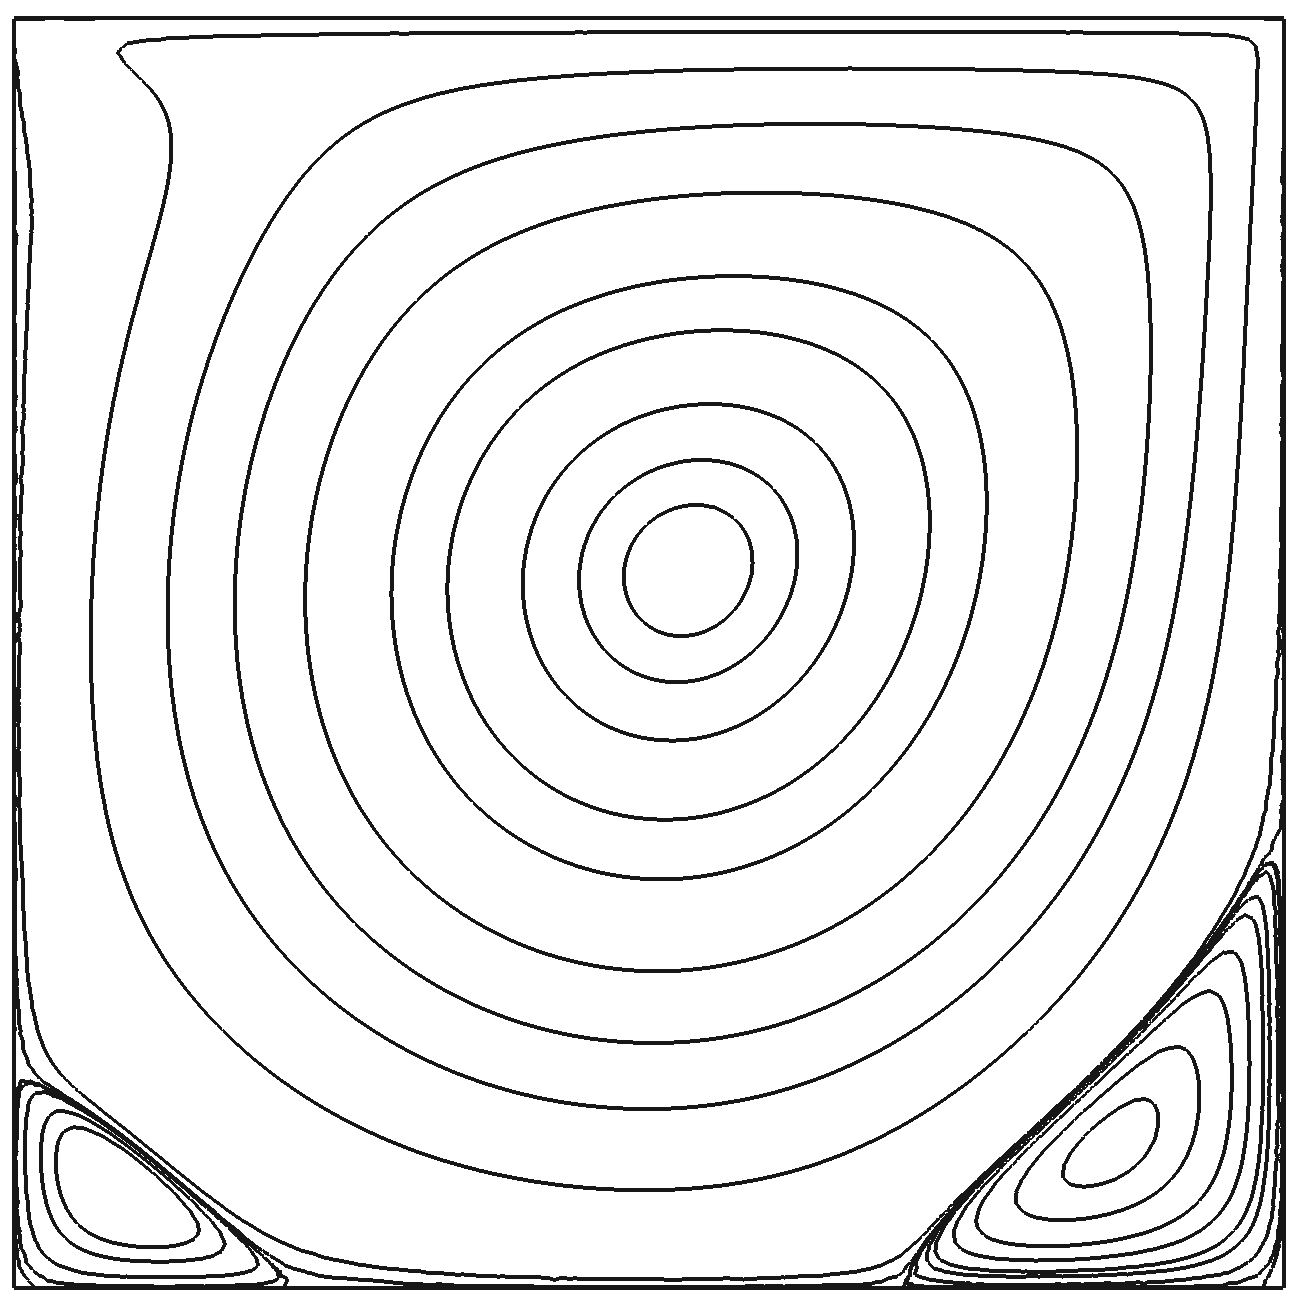
\includegraphics[width=0.4\textwidth]{./driven_cavity/driven_cavity_streamfunction.png}
\caption{Streamfunction contours in converged solution for $h=1/128$.}
\end{figure}
% end my slide
\end{frame}

\begin{frame}
    \frametitle{Lid--Driven Cavity - Output}
\begin{figure}
\centering
\subfigure[vorticity contours in converged solution for \mbox{$h=1/128$}]{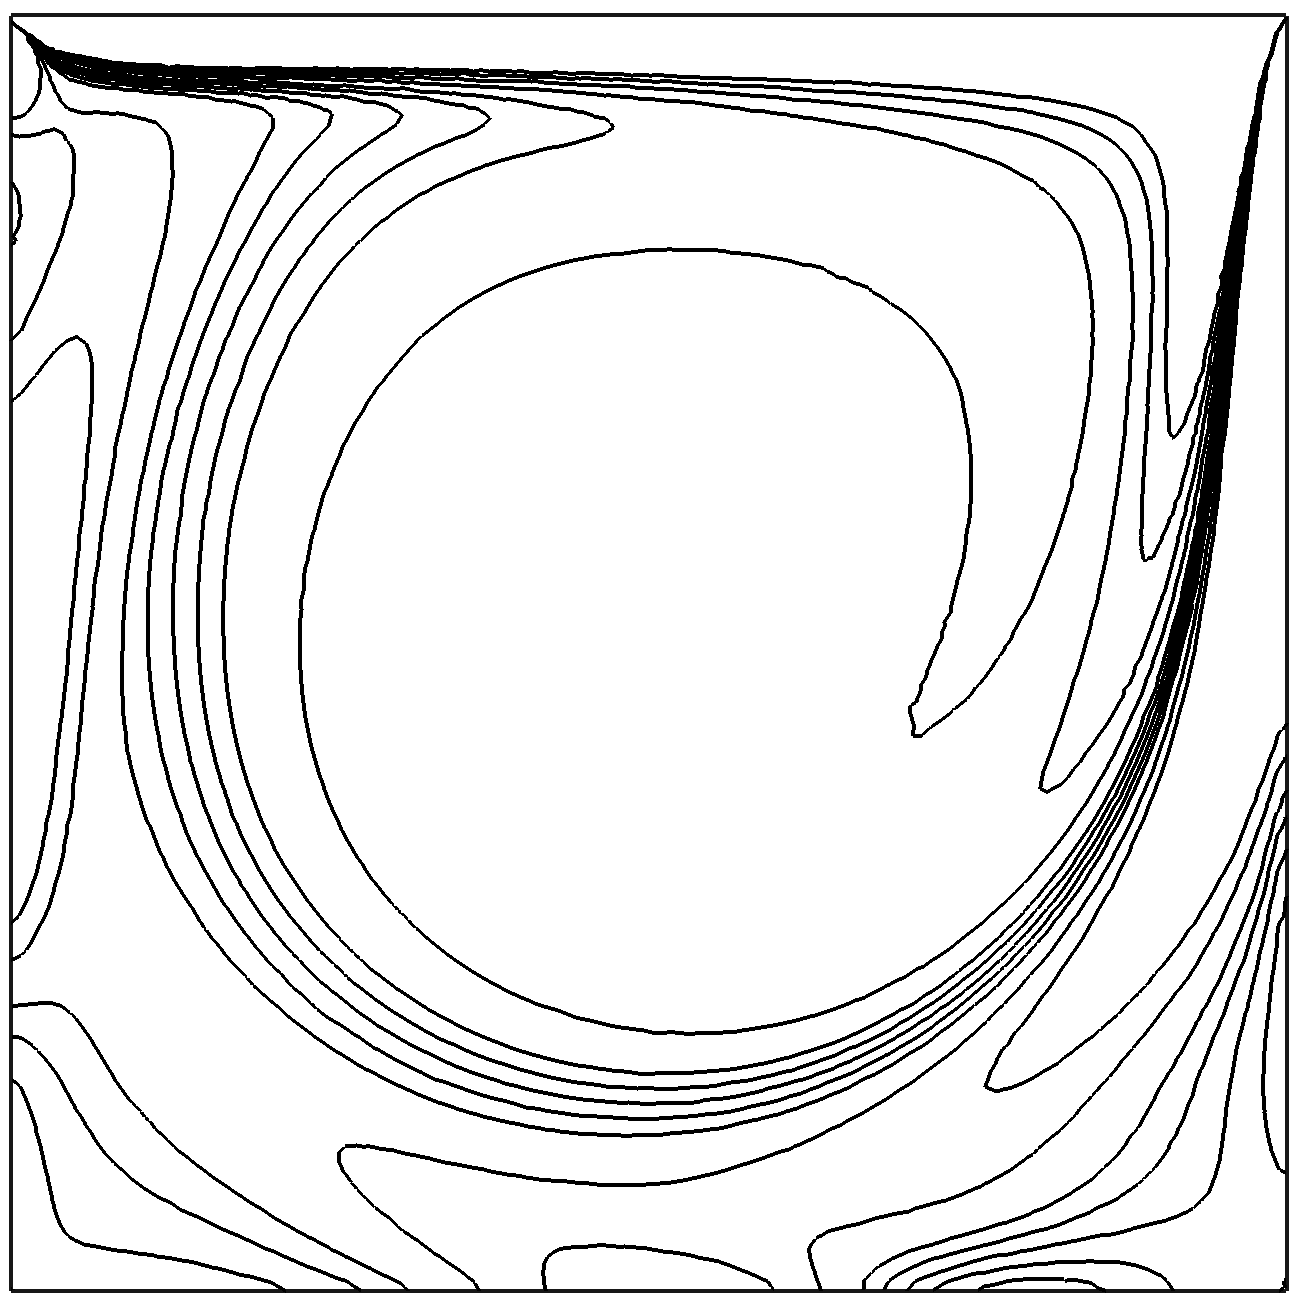
\includegraphics[width=0.35\textwidth]{./driven_cavity/driven_cavity_vorticity.png}}
\hspace{10mm}
\subfigure[error vs. mesh spacing for various metrics from the literature]{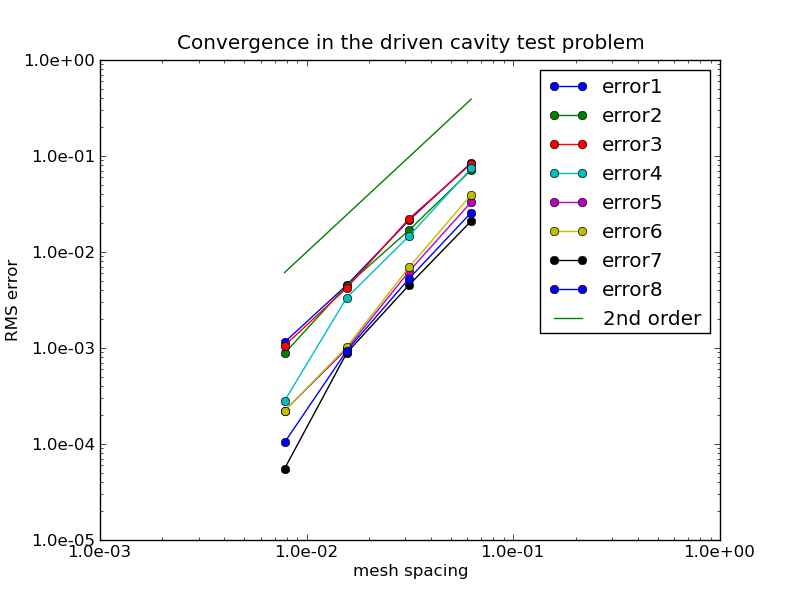
\includegraphics[width=0.45\textwidth]{./driven_cavity/driven_cavity_error_plot.png}}
\caption{The error metrics are described in the manual, section 10.4.}
\end{figure}
\end{frame}

\begin{frame}
  \frametitle{Lid--Driven Cavity - Exercises}
\begin{itemize}
\item What about mesh adaptivity?
\item Boundary condition on the lid is set to avoid issues in the upper corners. What happens if we modify this? Use a small mesh first!
\item What happens at higher $Re$?
\item What happens to wall clock time if you run in parallel?
\end{itemize}
\end{frame}






